\chapter{Fundamental Algoritma}\label{ch:app1}
\section{Variabel}
Variabel merupakan tempat penyimpanan data. 
\begin{contoh}
	\textbf{Penggunaan variabel}\\
	$a = 5 \rightarrow$ Memasukkan nilai 5 ke variabel `$a$'.\\
	$b = 7 \rightarrow$ Memasukkan nilai 7 ke variabel `$b$'.\\
	$a = b \rightarrow$ Memasukkan nilai variabel `$b$' ke variabel `$a$'. Kedua variabel sekarang bernilai 7.\\
	$a = b = 9 \rightarrow$ Memasukkan nilai 9 ke variabel `$a$' dan `$b$'.\\
\end{contoh}



\FloatBarrier
\section{Array}
Array merupakan kumpulan dari variabel. Satu array bisa menampung beberapa data. Gambar \ref{fig:illustrasiArray} menunjukkan illustrasi dari sebuah array yang berkapasitas $j$.
\begin{center}
	\begin{figure}[htbp]%
		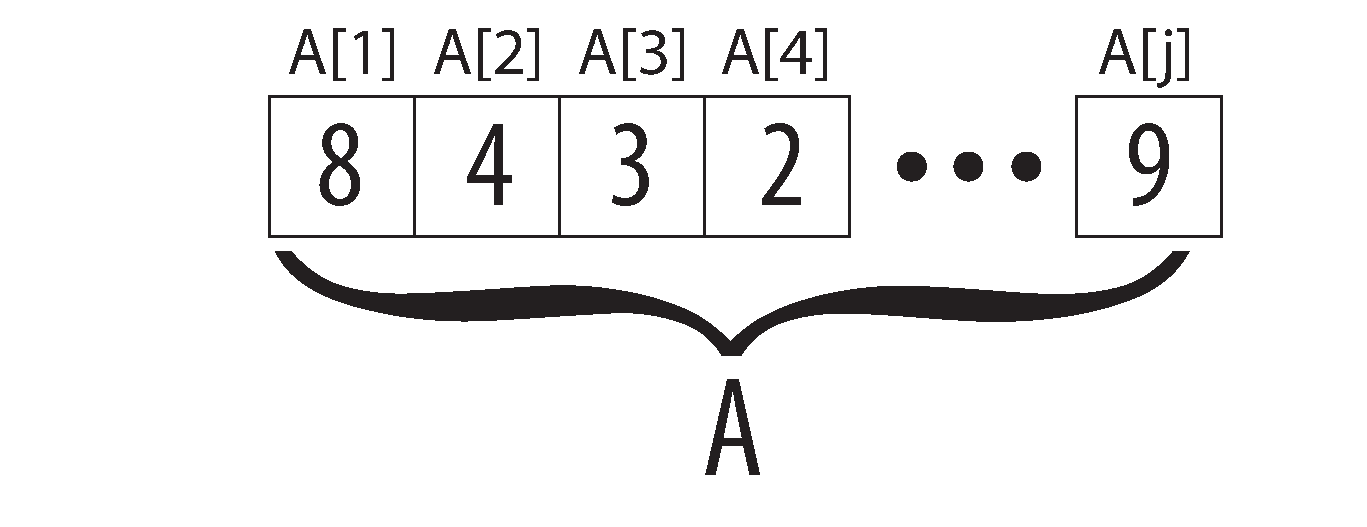
\includegraphics[scale=0.4]{fig/Array.eps}%
		\caption{Illustrasi Array}%
		\label{fig:illustrasiArray}%
	\end{figure}
\end{center}
\begin{contoh}
	\textbf{Penggunaan array}\\
	$A[i] \rightarrow$ Mengakses lokasi ke $i$ dari array yang bernama $A$.\\
	$A[4] \rightarrow$ Mengakses lokasi ke $4$ dari array yang bernama $A$.\\
	$A[i..j] \rightarrow$ Menandakan kumpulan isi array $A$ yang terdiri dari elemen $A[1],\ A[2],\ A[3],\ \ldots,\ A[j]$.\\
	$A[4] = 5 \rightarrow$ Memasukkan nilai 5 ke lokasi ke 4 dari array $A$.\\
	$b = A[4] \rightarrow$ Memasukkan nilai lokasi ke 4 dari array $A$ ke variabel $b$. 
	$A.length \rightarrow$ Menandakan besar/panjang dari array $A$.
\end{contoh}





\section{IF..THEN..ELSE}
Instruksi IF..THEN..ELSE disebut juga sebagai instruksi percabangan. 

\begin{contoh}
	\textbf{Blok IF..THEN..ELSE}
	\begin{algorithm}[H]
		\caption{Satu Blok IF}
		\begin{algorithmic}[1]
		\IF{$x > 4$} 
			\STATE $y = 5$ \COMMENT{Perintah ini hanya dijalankan jika nilai $x > 4$.}
		\ENDIF
		\end{algorithmic}
	\end{algorithm}
	\begin{algorithm}[H]
		\caption{Satu Blok IF dan ELSE}
		\begin{algorithmic}[1]
		\IF{$x > 4$} 
			\STATE $y = 5$ \COMMENT{Perintah ini hanya dijalankan jika nilai $x > 4$.}
		\ELSE
			\STATE $y = 6$ \COMMENT{Perintah ini hanya dijalankan jika nilai $x \leq 4$.}
		\ENDIF
		\end{algorithmic}
	\end{algorithm}
	\begin{algorithm}[H]
		\caption{Satu Blok IF..THEN..ELSE}
		\begin{algorithmic}[1]
		\IF{$x > 4$} 
			\STATE $y = 5$ \COMMENT{Perintah ini hanya dijalankan jika nilai $x > 4$.}
		\ELSIF{$x > 2$}
			\STATE $y = 8$ \COMMENT{Perintah ini hanya dijalankan jika nilai $2 < x < 4$.}
		\ELSE
			\STATE $y = 6$ \COMMENT{Perintah ini hanya dijalankan jika nilai $x \leq 4$.}
		\ENDIF
		\end{algorithmic}
	\end{algorithm}
\end{contoh}




\section{FOR}
Instruksi FOR disebut sebagai instruksi perulangan.
\begin{contoh}
	\textbf{Berbagai contoh penggunaan FOR}
	\begin{algorithm}[H]
	\caption{Perulangan 1 sampai 5}
		\begin{algorithmic}[1]
		\FOR{$i=1$ \TO $5$}
			\STATE print $i$
		\ENDFOR
		\STATE\COMMENT{Maka yang dicetak adalah 1 2 3 4 5}
		\STATE\COMMENT{Nilai $i$ terakhir yang tidak dicetak adalah 6}
		\end{algorithmic}
	\end{algorithm}
	\begin{algorithm}[H]
	\caption{Perulangan 5 sampai 1}
		\begin{algorithmic}[1]
		\FOR{$i=5$ \textbf{down to} $1$}
			\STATE print $i$
		\ENDFOR
		\STATE\COMMENT{Maka yang dicetak adalah 5 4 3 2 1}
		\end{algorithmic}
	\end{algorithm}
	\begin{algorithm}[htbp]
	\caption{Perulangan 1 sampai 5 pertambahan 2}
		\begin{algorithmic}[1]
		\FOR{$i=1$ \TO $5$ \textbf{by} 2}
			\STATE print $i$
		\ENDFOR
		\STATE\COMMENT{Maka yang dicetak adalah 1 3 5}
		\end{algorithmic}
	\end{algorithm}
\end{contoh}




\section{WHILE}
Instruksi WHILE merupakan instruksi perulangan yang berfungsi sama dengan instruksi FOR tetapi dengan cara penulisan yang berbeda.

\begin{contoh}
\textbf{Berbagai contoh penggunaan WHILE}
	\begin{algorithm}[H]
		\caption{Blok WHILE sederhana}
		\begin{algorithmic}[1]
			\STATE $i=1$
			\WHILE{$i<10$}
			\STATE print $i$
			\STATE $i=i+1$
		\ENDWHILE
		\end{algorithmic}
	\end{algorithm}
	
	\begin{algorithm}[H]
		\caption{Blok WHILE dengan 2 kondisi}
		\begin{algorithmic}[1]
			\STATE $i=1$
			\STATE $j=3$
			\WHILE{$i<10$ \AND $j<15$}
			\STATE print $i$
			\STATE print $j$
			\STATE $i=i+1$
			\STATE $j=j+3$
		\ENDWHILE
		\end{algorithmic}
	\end{algorithm}
\end{contoh}




\section{Fungsi}
Fungsi merupakan sub-program yang ditujukan untuk menggantikan kode-kode yang berulang di suatu program atau sering dipanggil. Fungsi bisa mengembalikan sebuah nilai ataupun tidak mengembalikan sama sekali.

\begin{contoh}
	\textbf{Berbagai contoh penggunaan fungsi}
	\begin{algorithm}[H]
		\caption{KUADRAT($n$)}
		\begin{algorithmic}[1]
			\RETURN $n\times{}n$
		\end{algorithmic}
	\end{algorithm}
	
	\begin{algorithm}[H]
		\caption{CEK-GANJIL($n$)}
		\begin{algorithmic}[1]
			\IF{$n\%2\neq0$}
				\RETURN \TRUE
			\ELSE
				\RETURN \FALSE
			\ENDIF
		\end{algorithmic}
	\end{algorithm}
	
	\begin{algorithm}[H]
		\caption{PRINT($n$)}
		\begin{algorithmic}[1]
			\STATE print($n$)
		\end{algorithmic}
	\end{algorithm}
\end{contoh}



\section{Fungsi Rekursif}
Fungsi rekursif adalah fungsi yang memanggil dirinya sendiri. Fungsi rekursif memakan sumber daya memori lebih banyak daripada iteratif (tidak menggunakan fungsi melainkan menggunakan FOR/WHILE).

\begin{contoh}
	\begin{algorithm}[H]
		\caption{REKURSIF($n$)}
		\begin{algorithmic}[1]
			\IF{$n==1$}
				\RETURN $n*2$
			\ELSE
				\RETURN REKURSIF($n-1$)$\times{}$3
			\ENDIF
		\end{algorithmic}		
	\end{algorithm}
	
	Jika fungsi REKURSIF($n$) dimasukkan parameter 3 maka hasilnya adalah:\\
	\begin{math}
	REKURSIF(3) = REKURSIF(2)\times{}3\\
	REKURSIF(2) = REKURSIF(1)\times{}3\times{}3\\
	REKURSIF(1) = 1\times{}2\times{}3\times{}3\\
	\end{math}
\end{contoh}